
\section{Theoretical Minimum}

\subsection{Of classical physics}

\begin{answer}
	Closed systems can actually exist if the collection of objects under investigation do not interact with anything outside of the system.

	Consider the empty system $\emptyset$, an empty collection that contains no objects.
	The empty system is a closed system that actually exists.

	Implicit in establishing a closed system are the assumptions that all interactions with its objects are known and can be definitively measured.
	An open system is a system that interacts with objects outside the system.

	As a matter of logic, a system should be presumed closed and shown to be open.
	However, the failure to establish a system to be open does not suffice to definitively conclude the system is closed.
\end{answer}

% functions of states 
\begin{answer}
	Consider a system consisting of six states $S = \left\{1, 2, 3, 4, 5, 6\right\}$.

	A law is given by a function $S \xrightarrow{f} S$ that assigns each state in $S$ to the state that results from evolution under the law.

	If any law is allowed, then the set of laws is given by the set of all functions from $S$ to $S$.

	If a law must satisfy the conservation of information, then the set of laws that are possible for a six-state system can be classified by the set of functions
	\begin{align}
		C & = \left\{ f : S \to S \mid \forall y \in S, \exists!\ x \in S. f(x) = y \right\},
	\end{align}
	where each function has the property that each element in its codomain has a corresponding, unique element in the domain that is mapped to it and thus each such function in $C$ is a bijection.
	The number of such laws, given by the size $\left|C\right| = 6!$ of $C$, is $6 \times 5 \times 4 \times 3 \times 2 \times 1 = 720$.
	This is because any function $S \xrightarrow{f} S$ in $C$ can be defined by sampling from the space $S$ of outcomes six times without replacement.
\end{answer}

\begin{answer}
	Consider the infinite system $\left\{\cdots, -1, 0, +1, +2, \cdots\right\}$.

	Examples of dynamical laws that are allowable include those given by the following equations.
	\begin{align}
		N(n+1) = N(n) - 1 \quad
		N(n+1) = N(n) + 2 \quad
		N(n+1) = -1^{N(n)} N(n)
	\end{align}
	On the other hand, the dynamical law given by the equation $N(n+1) = N(n)^2$ is not allowed because it does not satisfy the conservation of information.
\end{answer}

\subsubsection{Spaces, Trigonometry}

\begin{answer}
	Some functions are plotted below.
	\begin{figure}
		
% sciences/science/assets/plot.tex

\begin{subfigure}{0.32\textwidth}\centering
	\begin{tikzpicture}
		\begin{axis}[width=1\linewidth, legend pos=north east, legend style={font=\tiny}]
			\addplot[variable=t]{t^4 + 3*t^3 - 12*t^2 + t - 6  };
			\addlegendentry{$f(t) = t^4 + 3t^3 - 12t^2 + t - 6$}
		\end{axis}
	\end{tikzpicture}
	\caption{Plot of $f(t)$}
\end{subfigure}
\hfill
\begin{subfigure}{0.32\textwidth}\centering
	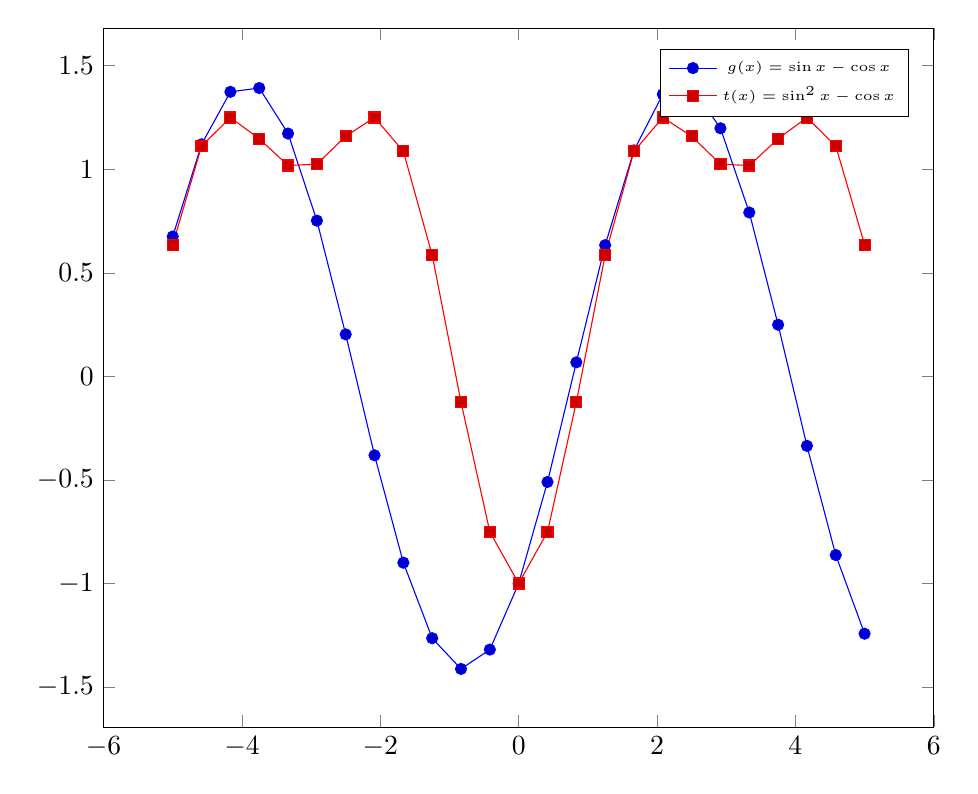
\begin{tikzpicture}
		\begin{axis}[trig format=rad, width=1\linewidth, legend pos=north east, legend style={font=\tiny}]
			\addplot{sin(x) - cos(x)};
			\addlegendentry{$g(x) = \sin x - \cos x$}
			\addplot{sin(x)^2 - cos(x)};
			\addlegendentry{$t(x) = \sin^2 x - \cos x$}
		\end{axis}
	\end{tikzpicture}
	\caption{Plot of $g(x)$ and $t(x)$}
\end{subfigure}
\hfill
\begin{subfigure}{0.32\textwidth}\centering
	\begin{tikzpicture}
		\begin{axis}[width=1\linewidth, legend pos=north east, legend style={font=\tiny}]
			\addplot[variable=\alpha]{e^(\alpha) + \alpha * ln(\alpha)};
			\addlegendentry{$\theta(\alpha) = e^\alpha + \alpha \ln \alpha$}
		\end{axis}
	\end{tikzpicture}
	\caption{Plot of $\theta(\alpha)$}
\end{subfigure}


		\caption{Plots of functions}
	\end{figure}
\end{answer}

\begin{answer}
	The rule for vector subtraction is to add the augend add the result of reversing the direction of the addend.

	Any vectors $\vec{A}$ and $\vec{B}$ satisfy the following equation.
	\begin{align}
		\vec{A} - \vec{B} & = \vec{A} + \left(-\vec{B}\right)
	\end{align}
\end{answer}

\begin{answer}
	For any vector $\vec{A}$, the magnitude $\left| \vec{A} \right| = \sqrt{A_x^2 + A_y^2 + A_z^2}$ of $\vec{A}$ satisfies the following equations:
	\begin{align}
		\vec{A} \cdot \vec{A} & = A_x A_x + A_y A_y + A_z A_z & = \left| \vec{A} \right|^2.
	\end{align}
\end{answer}

\begin{answer}
	Let $\left(A_x = 2, A_y = -3, A_z = 1\right)$ and $\left(B_x=-4, B_y=-3, B_z=2\right)$.

	The magnitude $\left|\vec{A}\right| = \sqrt{2^2 + (-3)^2 + 1^2}$ of $\vec{A}$ is $\left|\vec{A}\right| = \sqrt{4+9+1} = \sqrt{14}$.
\end{answer}

